\documentclass{standalone}
\usepackage{graphicx, standalone}
\usepackage[compat=1.1.0]{tikz-feynman}
\usepackage{tikz}
\usepackage{amsmath, amssymb}
\usepackage{euler}
\usepackage{fontspec}
\setmainfont{MinionPro}
\usepackage{comment}

\renewcommand{\k}{\ensuremath\text{k}}
\newcommand{\kp}{\ensuremath\text{k}'}
\newcommand{\q}{\ensuremath\text{q}}

\renewcommand{\r}{\ensuremath\text{r}}

\newcommand{\ph}{\ensuremath\text{ph}}
\newcommand{\phbar}{\ensuremath\overline{\text{ph}}}
\newcommand{\pp}{\ensuremath\text{pp}}

\newcommand{\dens}{\ensuremath\text{d}}
\newcommand{\magn}{\ensuremath\text{m}}
\newcommand{\sing}{\ensuremath\text{s}}
\newcommand{\trip}{\ensuremath\text{t}}

\renewcommand{\ss}{\ensuremath\sigma\sigma}

\begin{document}

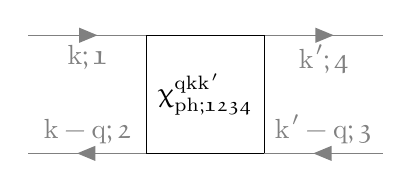
\begin{tikzpicture}[baseline=(current bounding box.center)]
	\begin{feynman}
		\vertex (a1);
		\vertex[right=of a1] (b1);
		\vertex[right=of b1] (c1);
		\vertex[right=of c1] (d1);
		\vertex[below=of a1] (a2);
		\vertex[right=of a2] (b2);
		\vertex[right=of b2] (c2);
		\vertex[right=of c2] (d2);		

		\node at ($(b1)!0.5!(c2)$) {$\chi^{\q\k\kp}_{\ph;\mathfrak{1234}}$};	
		
		\diagram* {
			(a1) -- [fermion, gray, edge label'=$\k;\mathfrak{1}$] (b1) -- (c1) -- [fermion, gray, edge label'=$\kp;\mathfrak{4}$] (d1),
			(d2) -- [fermion, gray, edge label'=$\kp-\q;\mathfrak{3}$] (c2) -- (b2) -- [fermion, gray, edge label'=$\k-\q;\mathfrak{2}$] (a2),
			(b1) -- (b2),
			(c1) -- (c2),		
		};
	\end{feynman}
\end{tikzpicture}
\begin{tikzpicture}[baseline=(current bounding box.center)]
	\node{$=$};
\end{tikzpicture}
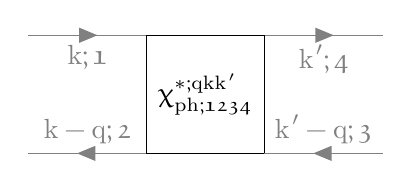
\begin{tikzpicture}[baseline=(current bounding box.center)]
	\begin{feynman}
		\vertex (a1);
		\vertex[right=of a1] (b1);
		\vertex[right=of b1] (c1);
		\vertex[right=of c1] (d1);
		\vertex[below=of a1] (a2);
		\vertex[right=of a2] (b2);
		\vertex[right=of b2] (c2);
		\vertex[right=of c2] (d2);		

		\node at ($(b1)!0.5!(c2)$) {$\chi^{*;\q\k\kp}_{\ph;\mathfrak{1234}}$};	
		
		\diagram* {
			(a1) -- [fermion, gray, edge label'=$\k;\mathfrak{1}$] (b1) -- (c1) -- [fermion, gray, edge label'=$\kp;\mathfrak{4}$] (d1),
			(d2) -- [fermion, gray, edge label'=$\kp-\q;\mathfrak{3}$] (c2) -- (b2) -- [fermion, gray, edge label'=$\k-\q;\mathfrak{2}$] (a2),
			(b1) -- (b2),
			(c1) -- (c2),		
		};
	\end{feynman}
\end{tikzpicture}
\raisebox{-2cm}{\hspace{-3.675cm}%
\begin{tikzpicture}[baseline=(current bounding box.center)]
	\node{$-$};
\end{tikzpicture}
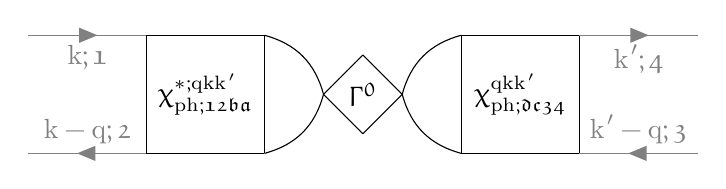
\begin{tikzpicture}[baseline=(current bounding box.center)]
	\begin{feynman}
		\vertex (a1);
		\vertex[right=of a1] (b1);
		\vertex[right=of b1] (c1);
		\vertex[right=of c1] (d1);
		\vertex[below=of a1] (a2);
		\vertex[right=of a2] (b2);
		\vertex[right=of b2] (c2);
		
		\vertex (x) at ($(c1)!0.5!(c2)$);
		\vertex[right=0.75cm of x] (i1);
		\vertex[right=1cm of i1] (i3);
		\vertex (i2) at ($(i1)+(0.5,0.5)$);
		\vertex (i4) at ($(i1)+(0.5,-0.5)$);
		\vertex[right=0.75cm of i3] (y);
		
		\vertex[above=0.75cm of y] (d1);
		\vertex[right=of d1] (e1);
		\vertex[right=of e1] (f1);
		\vertex[below=of d1] (d2);
		\vertex[right=of d2] (e2);
		\vertex[right=of e2] (f2);

		\node at ($(b1)!0.5!(c2)$) {$\chi^{*;\q\k\kp}_{\ph;\mathfrak{12ba}}$};
		\node at ($(d1)!0.5!(e2)$) {$\chi^{\q\k\kp}_{\ph;\mathfrak{dc34}}$};
		\node at ($(i1)!0.5!(i3)$) {$\Gamma^{0}$};
		
		\diagram* {
			(a1) -- [fermion, gray, edge label'=$\k;\mathfrak{1}$] (b1),
			(b2) -- [fermion, gray, edge label'=$\k-\q;\mathfrak{2}$] (a2),
			(b1) -- (c1) -- (c2) -- (b2) -- (b1),
			(i1) -- (i2) -- (i3) -- (i4) -- (i1),
			(c1) -- [bend left=30] (i1),
			(c2) -- [bend right=30] (i1),	
			(i3) -- [bend left=30] (d1),
			(i3) -- [bend right=30] (d2),	
			(d1) -- (e1) -- (e2) -- (d2) -- (d1),
			(f2) -- [fermion, gray, edge label'=$\kp-\q;\mathfrak{3}$] (e2),
			(e1) -- [fermion, gray, edge label'=$\kp;\mathfrak{4}$] (f1),
		};
	\end{feynman}
\end{tikzpicture}}

\end{document}